\beginsong{Bajuschki baju}[wuw={Michail Jurgewitsch Lermontow, ca. 1840, deutsche Übersetung von J.v. Günther}, pfii={103}, pfiii={39}, index={Schlaf, mein Bub}]

\beginverse
\endverse
\centering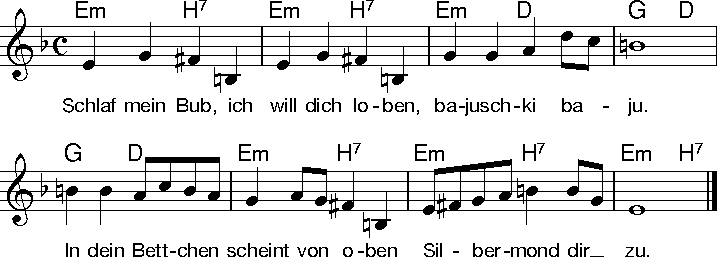
\includegraphics[width=1\textwidth]{Noten/Lied007.pdf}	

\beginverse
\[Em]Durch die \[H7]Felsen, \[Em]durch die \[H7]Lande, \[Em]strömt des \[D]Tereks \[G]Flut. \[D]
\[G]Der Tsche\[D]tschene \[Em]schleicht am \[H7]Strande, \[Em]schleift sein \[H7]Messer \[Em]gut. \[H7]
\endverse

\beginverse
^Doch dein ^Vater ^ist ein ^Reiter, ^greift ihn ^auf im ^Nu!  ^
^Schlaf, mein ^Kind, ^schlaf ruhig ^weiter, ^bajusch^ki ba^ju. ^
\endverse

\beginverse
^Du wächst ^auf, die ^Zeit hat ^Flügel, ^wirst ein ^Held wie ^er;  ^
^Mutig ^steigst du ^in die ^Bügel, ^greifst nach ^dem Ge^wehr. ^
\endverse

\beginverse
^Sticken ^werde ^ich mit ^Seide ^Sattel ^dir und ^Schuh'. ^
^Schlaf mein ^Kindchen, ^meine ^Freude, ^bajusch^ki ba^ju. ^
\endverse

\beginverse
^Ein Ko^sak wirst ^du bei^zeiten ^und ein ^Held ge^nannt; ^
^wirst du ^einstmals ^von mir ^reiten, ^winkst du ^mit der ^Hand. ^ 
\endverse

\beginverse
^Denk, stehst ^du im ^Kampfes^feuer, ^meiner ^immer^zu. ^
^Schlaf mein ^Liebling, ^mir so ^teuer, ^bajusch^ki ba^ju. ^ \[Em]
\endverse

\endsong

\beginscripture{}
''Bajuschki baju'' ist russisch und bedeutet "Heia heia". Das Lied entstand zur Zeit des Kaukasuskrieges (1817 - 1864), in dem das Russische Kaiserreich versuchte, die Kontrolle über den von Tscherkessen und Tschertschenen besetzten Nordkaukasus zu erlangen.
\endscripture

\begin{intersong}
\ifthenelse{\boolean{pics}}{
    \ThisLRCornerWallPaper{1}{Bilder/bajuschkibaju_irena.png}
}{}
\end{intersong}